\documentclass{article}
\usepackage[utf8]{inputenc}
%\usepackage[francais]{babel}
\usepackage[T1]{fontenc}
\usepackage{graphicx}
\usepackage{eurosym}
\usepackage{verbatim}
\usepackage{amsmath, amsthm}
\usepackage{latexsym}
\usepackage{amssymb}
\usepackage{tabularx}
\usepackage{setspace}
\usepackage{listings}
\usepackage{geometry}
\usepackage{fancyhdr}
%\usepackage{enumitem}
\usepackage{colortbl}
%\usepackage[dvipsnames]{xcolor}
\usepackage{booktabs}
%\usepackage{moreverb}

\DeclareMathAlphabet{\mathonebb}{U}{bbold}{m}{n}
\newcommand{\one}{\ensuremath{\mathonebb{1}}}

\usepackage{color}
%\usepackage{multirow}
%\usepackage{float}
\definecolor{gris25}{gray}{0.75}
\usepackage{colortbl}
\usepackage{fancyhdr}
\usepackage{amsmath,amsfonts,amssymb}
%\usepackage{titlesec}
%\usepackage{supertabular}
\usepackage{longtable}

\usepackage{caption}
\usepackage{subcaption}


\usepackage{listings}
\definecolor{dkgreen}{rgb}{0,0.4,0}
\definecolor{gray}{rgb}{0.5,0.5,0.5}
\definecolor{mauve}{rgb}{0.58,0,0.82}

%\usepackage{algorithm2e}

% marges,etc.
%\usepackage{a4wide}
\hoffset -1cm
\voffset -2cm
\textheight 23cm
\headheight 1cm
\headsep 1cm
\topmargin 0cm
\textwidth 16cm

%pour les couleurs
\usepackage{color}
\definecolor{mycolor}{rgb}{0.06,0.32,0.39}

%liens dans le corps du texte
\usepackage{hyperref}
\hypersetup{
    colorlinks=true,
    linkcolor=blue,
    filecolor=magenta,
    urlcolor=blue,
}

\urlstyle{same}

\definecolor{dkyellow}{cmyk}{0, 0, 0.2, 0}
\lstset{
  language=Python,                % the language of the code
  basicstyle= \footnotesize,      % the size of the fonts that are used for the code
  numbers=left,                   % where to put the line-numbers
  numberstyle=\tiny\color{gray},  % the style that is used for the line-numbers
  stepnumber=2,                   % the step between two line-numbers. If it's 1, each line
                                  % will be numbered
  showspaces=false,               % show spaces adding particular underscores
  showtabs=false,                 % show tabs within strings adding particular underscores
  frame=single,                   % adds a frame around the code
  rulecolor=\color{black},        % if not set, the frame-color may be changed on line-breaks within not-black text (e.g. commens (green here))
  tabsize=2,                      % sets default tabsize to 2 spaces
  captionpos=b,                   % sets the caption-position to bottom
  breaklines=true,                % sets automatic line breaking
  breakatwhitespace=false,        % sets if automatic breaks should only happen at whitespace
  keywordstyle=\color{blue},      % keyword style
  commentstyle=\color{dkgreen},   % comment style
  stringstyle=\color{mauve},       % string literal style
  backgroundcolor=\color{white},      % choose the background color. You must add \usepackage{color}
}

\usepackage{array}
\newcolumntype{L}[1]{>{\raggedright\let\newline\\\arraybackslash\hspace{0pt}}m{#1}}
\newcolumntype{C}[1]{>{\centering\let\newline\\\arraybackslash\hspace{0pt}}m{#1}}
\newcolumntype{R}[1]{>{\raggedleft\let\newline\\\arraybackslash\hspace{0pt}}m{#1}}

\usepackage{xcoffins}
\NewCoffin\tablecoffin
\NewDocumentCommand\Vcentre{m}
  {%
    \SetHorizontalCoffin\tablecoffin{#1}%
    \TypesetCoffin\tablecoffin[l,vc]%
  }

% mise en forme des en-têtes et pieds de page
\usepackage{fancyhdr}
    \rhead{\markright}
    \lfoot{\scriptsize{Peter NAYLOR - Juin, 2016}}
    \cfoot{\thepage}
    \rfoot{ \scriptsize{1st year PhD report}}
    \renewcommand{\headrulewidth}{0.6pt}
    \renewcommand{\footrulewidth}{0.5pt}
    \makeatletter
         \def\headrule{{\if@fancyplain\let\headrulewidth\plainheadrulewidth\fi
              \color{mycolor}\hrule\@height\headrulewidth\@width\headwidth \vskip-\headrulewidth}}
         \def\footrule{{\if@fancyplain\let\footrulewidth\plainfootrulewidth\fi
              \vskip-\footruleskip\vskip-\footrulewidth
              \color{mycolor}\color{mycolor}\hrule\@width\headwidth\@height\footrulewidth\vskip\footruleskip}}
    \makeatother
\pagestyle{fancy}




\begin{document}
%%%%%%%%%%%%%%%%%%%%%%%%%%%%%%%%%%%%%%%%%%%%%%%%%%%%%%%%%%%%%%%
\begin{titlepage}

%  \begin{center} 
%    \textsc{ENSAE ParisTech}\\
%    ---\\
%    Année 2013--2014
%  \end{center}
  
\begin{center}

\includegraphics[width=0.3\textwidth]{Mines_ParisTech.png} 

\includegraphics[width=0.3\textwidth]{CURIE.jpg}

\includegraphics[width=0.3\textwidth]{INSERM.jpg}
\end{center}

\vspace{\stretch{1}}
 
\noindent
\begin{center}
\textcolor{mycolor}{\rule{16cm}{0.6pt}}\\
\vspace{0.1cm}
\hrule height 2pt
\vspace{0.1cm}
\textcolor{mycolor}{\rule{16cm}{0.6pt}}\\
\end{center}
  \begin{center} \bfseries\Huge
Towards image-based cancer signatures from histopathology data
  \end{center}
  \begin{center} \huge
   First year report
  \end{center}
\begin{center}
\textcolor{mycolor}{\rule{16cm}{0.6pt}}\\
\vspace{0.1cm}
\hrule height 2pt
\vspace{0.1cm}
\textcolor{mycolor}{\rule{16cm}{0.6pt}}\\
\end{center}
  
  \vspace{\stretch{2}}
   \begin{center}  \large
\textit{Supervisor} : \textsc{T. Walter and F. Reyal}. \\
\textit{Units:} \textsc{Center for Computational Biology and UMR900}

   \end{center}
     
  \vspace{\stretch{3}}
  \begin{center} \Large
  Peter \textsc{Naylor}
  \end{center}

  \vspace{\stretch{4}}

  \begin{center}  \large
    June 2016
  \end{center}

\end{titlepage}
%%%%%%%%%%%%%%%%%%%%%%%%%%%%%%%%%%%%%%%%%%%%%%%%%%%%%%%%%%%%




\newpage
\tableofcontents
\newpage

\section{Introduction}

\subsection{Context}

\subsection{PhD subject}

\section{November 2015 - January 2016: MitoCheck Project}

\section{January 2016 - April 2016: Camelyon2016 challenge}

This Challenge is organized in conjunction with and with the support of the 2016 IEEE International Symposium on Biomedical Imaging  (ISBI-2016) and this the first challenge using whole-slide images in histopathology. This challenge fitted particularly well with my PhD time table as the data used in this challenge is very similar to the data acquired by F. Reyal. Our final ranking was not very satisfying as we did not achieve good results. This work was done with the help of V. Machairas, T. Walter and E. Decenciere. A website was made for the purpose of this challenge, \url{http://camelyon16.grand-challenge.org/home/}.

\subsection{Context}
The goal of this challenge is to evaluate new and existing algorithms for automated detection of metatases in hematoxylin and eosin (HE) stained whole-slide images of lymph node sections, see figure \ref{LymphNode} This task has a high clinical relevance but requires large amounts of reading time from pathologists. Therefore, a successful solution would hold great promise to reduce the workload of the pathologists while at the same time reduce the subjectivity in diagnosis. The Camelyon2016 challenge will focus on sentinel lymph nodes of breast cancer patients and 2 large datasets have been provided from both the Radboud University Medical Center (Nijmegen, the Netherlands), as well as the University Medical Center Utrecht (Utrecht, the Netherlands). The focus on lymph nodes of breast cancer patients is not arbitrary, lymph node metastases occur in most cancer types (e.g. breast, prostate, colon). Lymph nodes are small glands that filter lymph, the fluid that circulates through the lymphatic system. The lymph nodes in the underarm are the first place breast cancer is likely to spread. Metastatic involvement of lymph nodes is one of the most important prognostic variables in breast cancer. Prognosis is poorer when cancer has spread to the lymph nodes.

\begin{figure}[!ht]
\centering
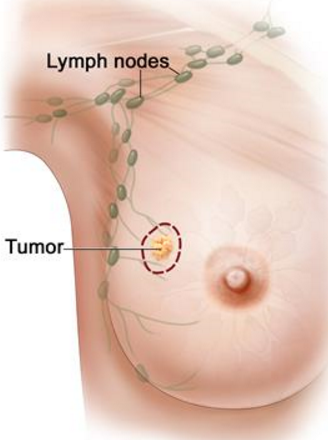
\includegraphics[width=0.3\textwidth]{Booby.png}
\caption{Lymph nodes}
\label{LymphNode}
\end{figure}

\subsubsection*{Data}
The data in this challenge contains a total of 400 whole-slide images (WSIs) of sentinel lymph node from two independent datasets collected in Radboud University Medical Center (Nijmegen, the Netherlands), and the University Medical Center Utrecht (Utrecht, the Netherlands). The training dataset consists of 270 WSIs of lymph node (160 Normal and 110 containing metastases). WSI are generally stored in a multi-resolution pyramid structure. WSI contain multiple downsampled versions of the original image. Each image in the pyramid is stored as a series of tiles, this file structure is to facilitate rapid retrieval of subregions of the image as one could not even open one at the highest resolution, see figure \ref{fig: Pyramid}. These compression technics are similar to those used by Google Earth and even use the same compression format, jpeg2000. Uncompressed, one image can reach up to 65 GB, the WSI have , at the highest resolution, a size of 96256 x 218624 pixels and have only 188 x 427 pixels at the lowest resolution.


\begin{figure}[!ht]
\centering
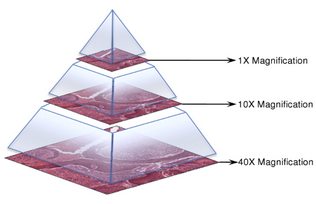
\includegraphics[width=0.5\textwidth]{pyramid.png}
\caption{Pyramid data Structure}
\textit{Between 8 and 10 different resolutions}
\label{fig: Pyramid}
\end{figure}


\subsection{Classification problem}
There were two evaluations and therefore two distinct scoreboards for this challenge. The first is slide based and can be seen as a binary classification, given a Whole-slide Images (WSI) we had to give a confidence score that this WSI contained metastases. The final score for this evaluation was given by the area under the curve (or ROC curve) asserted over 130 test slides. The second was a lesion-based evaluation, this evaluation was aimed to asses the metastases detection within a given slide. This within slide evaluation was measured vi a free-response receiver operating characteristic (FROC). This is similar to ROC analysis, except that the false positive rate on the x-axis is replaced by the average number of false positives per image. For this challenge, our detection will be considered a true positive, if the location of the detected region is within the annotated ground truth lesion. The FROC curve is defined as the plot of sensitivity versus the average number of false-positives per image. 

Due to limited time, we tackled these two evaluations as a pixel classification in supervised setting. Each pixel is described by a vector of features $x \in \mathbb{R}^P$. The training set is composed of a set of such vectors $x^T$,combined in the data matrix $X \in \mathbb{R}^{N \times P}$ and the corresponding labels $Y \in \{0,1\}^N$, provided by the challenge annotators. 
%The concatenation of all vectors is denoted by $X \in
The computational steps and design choices that had to be made can be categorized as follows: 
\begin{enumerate}
	\item Pre-processing of the stained whole-slide images.
	% Feature  extraction. Here, we used a pannel of color and texture
    %     descriptors, evaluated on superpixel regions.
	%\item Sampling strategies in order to derive a reasonably
    %      sized training data set. 
         \item Classification method: here we tested and adapted
           Random Forests and Support Vector Machines. 
         \item Post-processing of the probability map.
\end{enumerate}
%%---------------------------------------
%%---------------------------------------

%\begin{figure}[!ht]
%\centering
%
\includegraphics[width=\textwidth]{Camelyon16.png}
%\caption{Official logo}
%\label{Ol}
%\end{figure}
\subsection{Work pipeline}
Some of the decisions made in this section where a necessity due to the technological difficulties caused by the type of data. In figure \ref{PipelineCam}, I expose a graphic summarising the pre-processing step to the classification problem. The pre-processing step is not included in this graphic.

\begin{figure}[!ht]
\centering
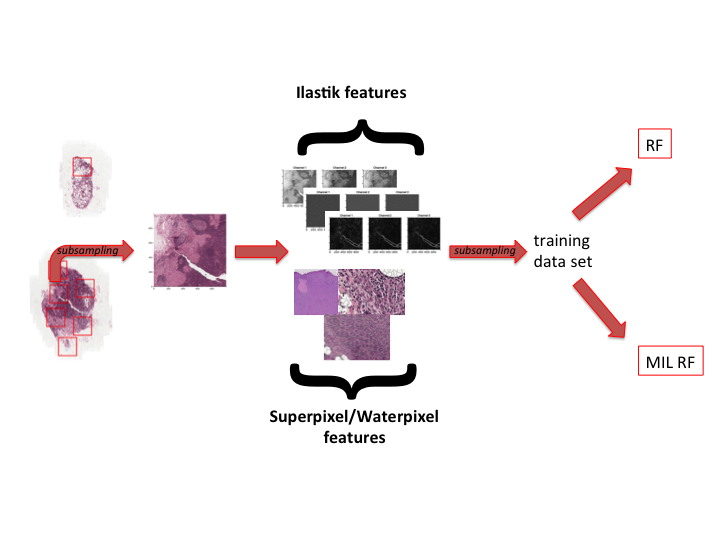
\includegraphics[width=\textwidth]{workflow.png}
\caption{Work pipeline for the Camelyon2016 project.}
\label{PipelineCam}
\end{figure}


\subsubsection*{Pre-processing}

In order to access relevant information in such a tiff file, we had to think careful as how to segment the whole image to have relevant patches, these patches were a necessity to process the information contained in the slide (Memory constraints). As a WSI is mostly composed of white, processing only the patches contain tissue were restrained. The method used relied on a threshold segmentation of the WSI at a low resolution in order to cover the whole image. Once the tissue areas were found, we extracted small patches at a very high resolution (resolution number 2) randomly from the WSI. 300 to 400 images of size 1000 x 1000 were extracted on average per WSI. We then applied color deconvolution \cite{deconvolution} to the smaller images in order to obtain a physicologically relevant representation
of the color information.  This was done in order to reduce the
computational burden for the subsequent steps.
%A set of 100 \textit{Superpixel-Adaptive Features} (SAF) were used to
%describe each pixel of the train and test image databases. As
%presented in \cite{saf}, these features are well suited for
%segmentation purposes as they are computed on superpixels, i.e. on a
%\textit{computational support} which adapts to the image
%content. 
%Here, we used \textit{waterpixels} \cite{waterpixels}, as they feature
%good adherence to real object boundaries and they are very fast to
%compute. In particular, this allowed us to calculate several
%superpixel partitions, therefore capturing information at different
%scales. 

On each image, we calculated a large panel of different features describing color
and texture of the images. For this, different operators were applied
on the images: identity; a set of operators from Mathematical
Morphology: erosion, opening, top hat and morphological gradient (different
sizes of structuring elements with V6 neighborhood); Haralick texture
features (averaged on all directions). We also applied a family of features based
on Gaussians: difference of gaussians (faster approximation of the
laplacian), eigenvalues of the structure tensor, eigenvalues of
hessian of gaussian based, this family of features are the same set found in the software Ilastik, see \cite{Ilastik}.

We evaluated these features on superpixel regions: we first calculated
a partition of the image into superpixels. Here, we used
\textit{waterpixels} \cite{waterpixels}, as they feature good
adherence to real object boundaries and they are very fast to
compute.  In particular, this allowed us to calculate several
superpixel partitions with different size parameters, therefore capturing
information at different scales. The features were then evaluated on
the superpixel regions (average values) at the different
scales. Altogether, we obtained 100 features for each pixel in this step. 

%The partition into waterpixels (with a given set of parameters values)
%was computed once and each pixel was assigned
%the average pixel value within the superpixel it belonged to. 
%
%In order to
%capture multiscale information, we repeated the process with
%waterpixels of different sizes ($step \in \left[ 15,20, 30\right]
%pixels$).\\ 
%
%%---------------------------------------
%%---------------------------------------
\subsubsection*{Classification model}
%%---------------------------------------
%%---------------------------------------
We investigated two classification methods: Random Forests and Support
Vector Machines with RBF kernels. The particularity of the
classification task was an extremely large number of samples ($N \sim  10^{10}$).
Consequently, we could not simply apply the learning algorithms on the
entire data set.  
\begin{enumerate}
\item {\it Random Forests (RF):} Having access to a very large number of
  samples allows us to modify the standard RF procedure. Random
  forests work best, if the individual trees are different from each
  other and cover ``different aspects'' of the data. This is normally
  achieved by boosting, and by randomly drawing the features to be
  considered. With the amount of annotated data we have here, we can
  afford presenting different data to each tree. We therefore generate
  different (but stratified) training sets for each tree of the Random
  Forest.  
\item {\it Support Vector Machines (SVM):} Training with large number
  of samples is generally problematic for non-liner SVM. We therefore
  downsampled the data presented to the classifier. In order to
  properly sample the feature space, we designed a hierarchical
  strategy, where we first apply k-means to each slide, and keep only
  a few representing data points for each cluster. This allowed us
  then to learn an SVM with and RBF kernel. 
\end{enumerate}

Once we have a trained classifier, this allowed us to predict on a WSI (via down-sampling) and to obtain probability maps corresponding (hopefully) to pixel based confidence map of each pixel belonging to a metastasis. Given the results on the cross-validation we choose a Random Forest model as it outperformed on F1-score metric and in accuracy. Also, the prediction probability maps on most slides were a lot less noisy than the ones acquired by the Support Vector Machine. The results and and parameter tuning are given in table \ref{Cross_val: RF}. We can also take a look at \ref{ProbabilityMapLocalMaxima} which is the output given by our algorithm for the test WSI number 2.

\subsubsection*{Post-processing}

Once we have the probability map of a WSI at a lower resolution we have to decide how to extract the information to better suit the two different tasks. One the one hand, for the slide base evaluation, as we choose a RF model, we could easily take the maximum value of the probability map as the confidence score of this WSI containing metastasis. On the other hand, for the lesion-based evaluation, it was difficult as we had to detect each distinct metastasis, but also not miss as little as possible. We proceeded as the following: we smoothed the image by applying a gaussian filter. The next step extracts local maxima within a connected component as to to reduce this connected region to a single data point. We can take a look at figure \ref{Detecting maxima} as an example of our metastasis location within a WSI.

\begin{figure}[!ht]
\centering
\begin{subfigure}{.33\textwidth}
  \centering
  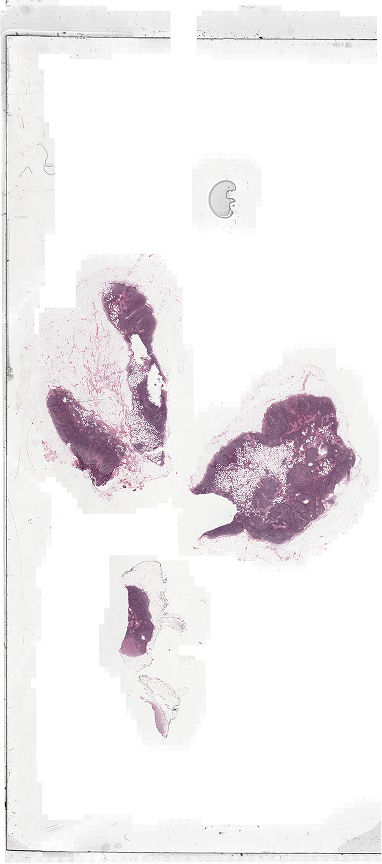
\includegraphics[width=\linewidth]{Test_002_whole.png}
  \caption{RGB raw data.}
  \label{fig:sub1}
\end{subfigure}%
\begin{subfigure}{.33\textwidth}
  \centering
  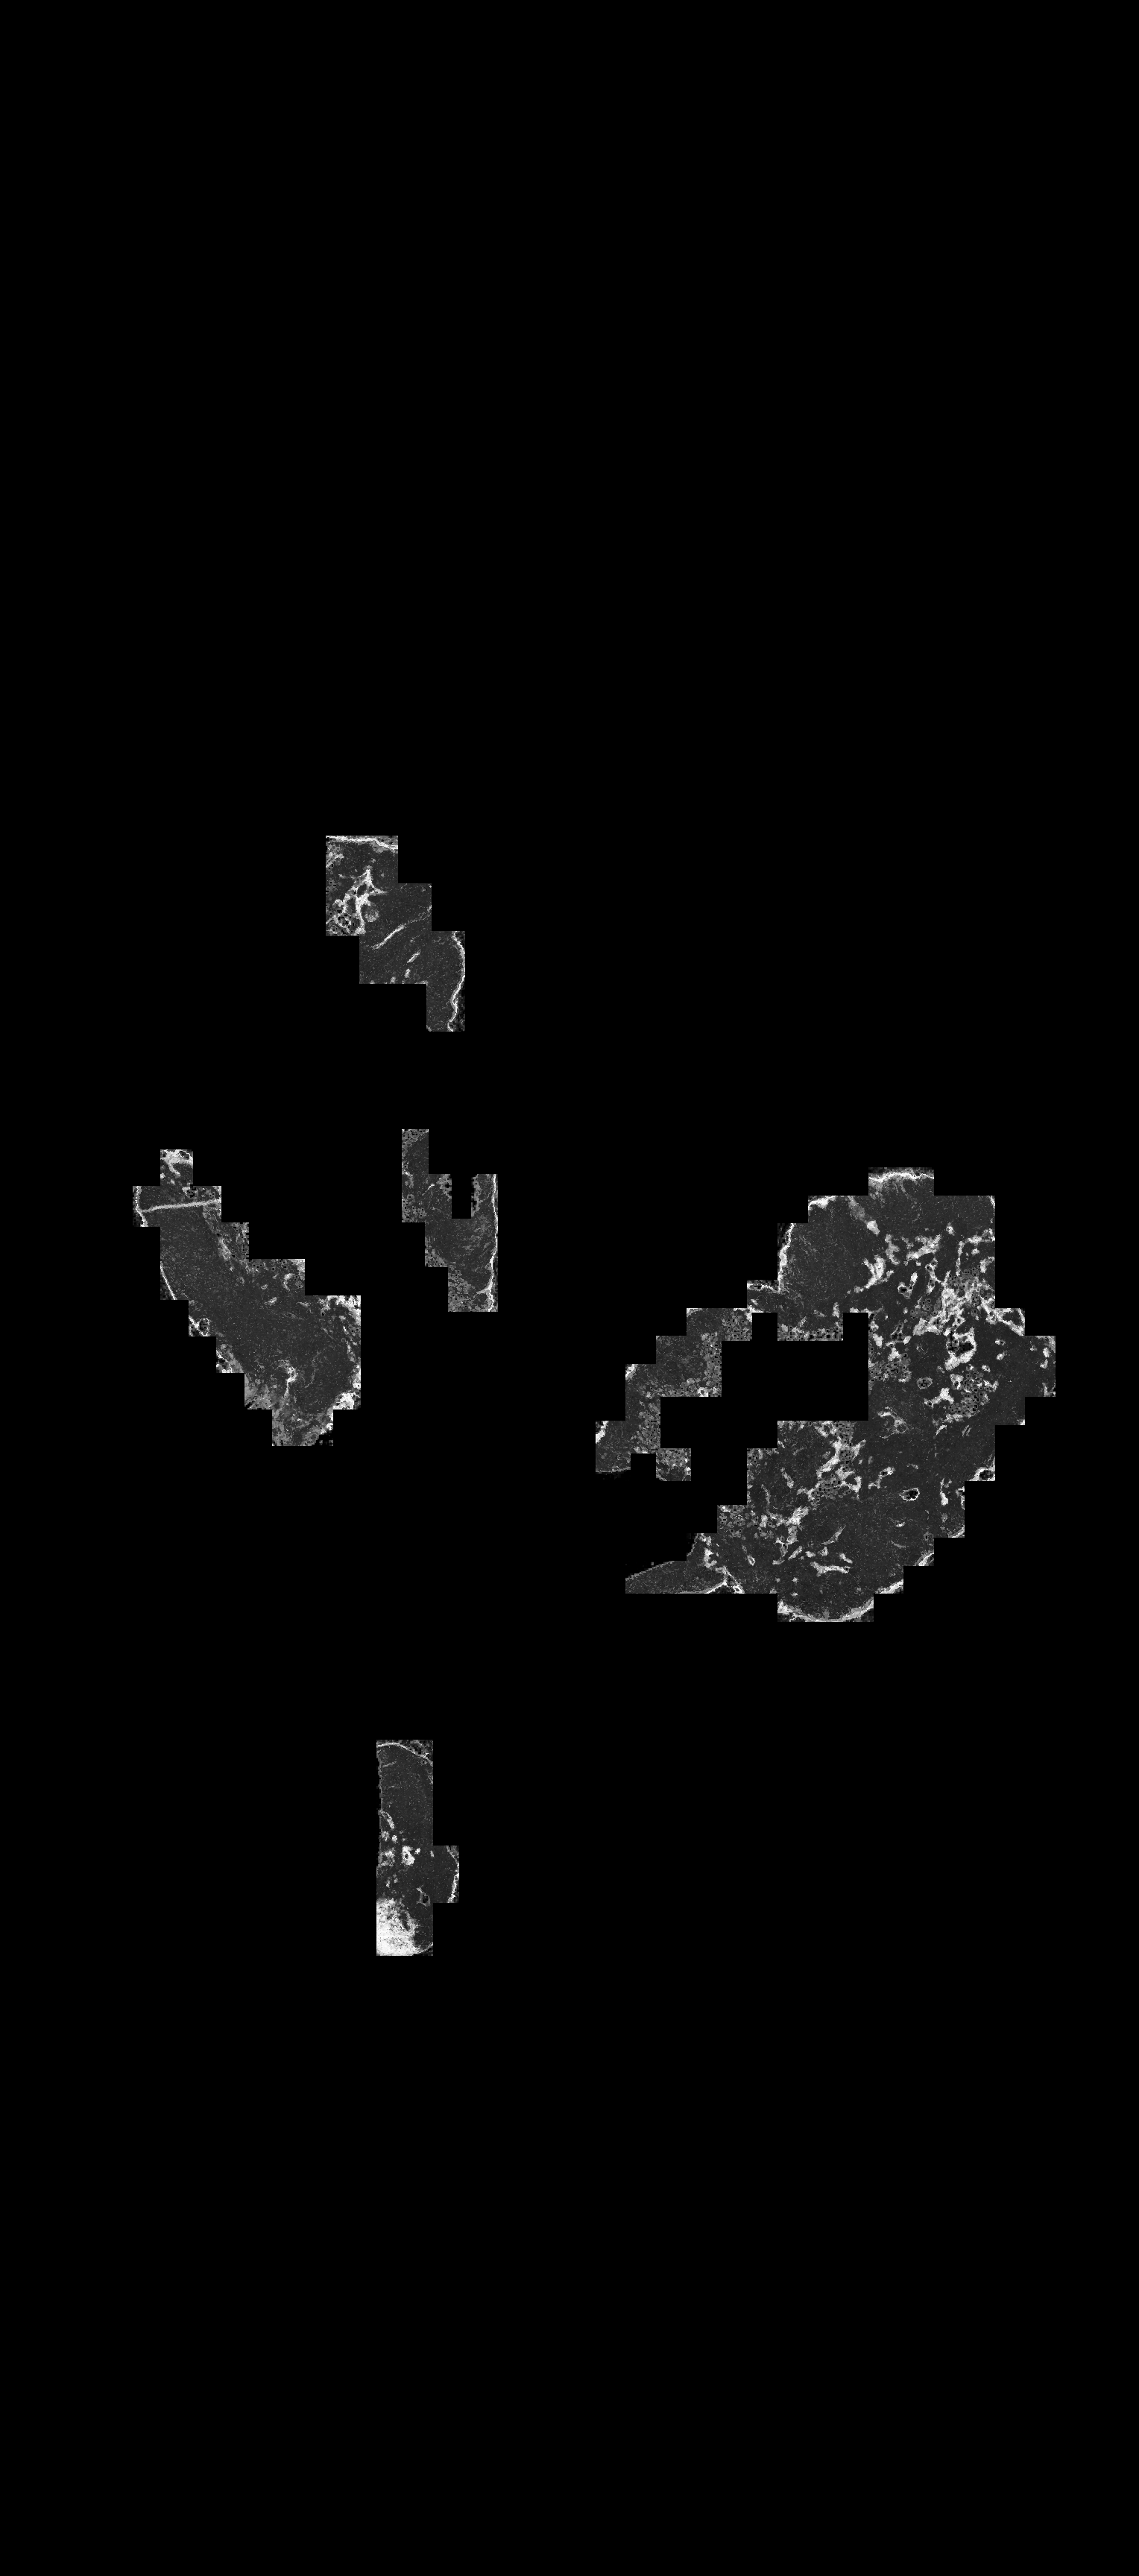
\includegraphics[width=\linewidth]{whole_probmap_Test_002.png}
  \caption{Probability map.}
  \label{ProbabilityMapLocalMaxima}
\end{subfigure}
\begin{subfigure}{.33\textwidth}
  \centering
  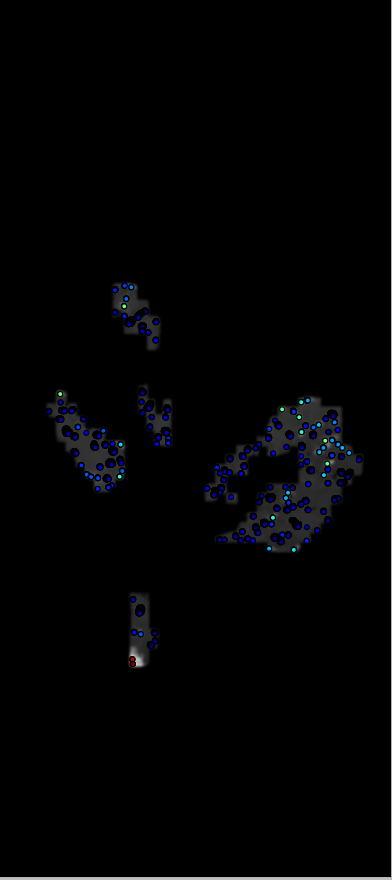
\includegraphics[width=\linewidth]{Detection.png}
  \caption{Metastasis confidence pin-points.}
  \label{Detecting maxima}
\end{subfigure}
\textit{For figure (c), blue is equal to a low confidence score whereas red means a high confidence.}
\caption{Evaluation whole slide image, test slide number 2.}
\label{fig:test}
\end{figure}

\subsubsection*{Technological difficulties}

Due to the very large size of each WSI, we encountered several difficulties due to data transfer. We have at our disposal 2 clusters, the cluster at Fontainebleau and the one in Curie. I used the one put at disposal by Les Mines at Fontainebleau. This cluster has 424 nodes with several machines of different capacities. However one issue seriously troubled us, before testing submitting many jobs to the cluster we performed tests on our local machine in order to access the computation time to evaluate the waiting time. From experience (not my own), it is normal to have a factor 2 or 3 in the computation time for a single job, how ever here we had a factor 100 in time. It took us a considerable amount of time to figure out what the problem was. It had nothing to do with the code, it was a problem of data transfer and in particular of transferring the data to a single node of the cluster. On our cluster, a node can access up to 125 MB / s, which 8 times slower than on my desktop computer. As we had tera bytes of data to transfer this was painfully slow. This limitation, explained only a week before the end of the challenge made every step more complicated. We had to have clear subsampling strategies in order to make the data as small and as relevant as possible. For instance, applying the color deconvolution in order to have only 2 color channels instead of 3 reduce immediately the size of the datasets by $\frac{1}{3}$. This computation limitation enforced us to not have fewer features, to not have as many experiences and tests as we initially wished. Another issue, related to data transfer is the evaluation scheme with respect to the tuning of each model, we couldn't use the same metric as the one in the challenge as this one implies predicting over a WSI, which was not possible in terms of time and of computation. So instead we had to maximize over the F1-score, see table \ref{Cross_val: RF}.

This challenge was very rewarding as the he taught me a huge amount about cluster policies, organisation and use!


\subsection{Challenge Results and ISBI 2016}

As I participated to this challenge it was interesting for me to be present to the presentations concerning it. We made 22 out of 23 on the first leader board and our ROC curve is displayed in figure \ref{Eval: ROC}. We reached 0.63\% of area under the curve. We ended last in the second score board as our post-processing phase was not reducing enough the amount of detected metastasis. To better explain this aspect, let's have a closer look at figure \ref{Detecting maxima}, on the lower part of the tumor we have two red point indicating that we have detected a metastasis with high confidence in that region. However their is two points, if we are mistaken this will lead to two false positives. It is also interesting to note that only 3 teams used classical methods to extract information from the WSI. The best of these three teams reached an area under the ROC curve of 0.76\% and finished 11. The 3rd team performing classical methods was last. After a brief discussion with the best performing team within classical extraction method, we hope that our method could reach 0.76\% with a better tuning, with respect to the feature, model parameters and model evaluation. However, all the other teams used Convolutionnal Neural Networks and achieved much better result than classical methods. This gave us clear view of my next study, deep neural networks.

\begin{figure}[!ht]
\centering
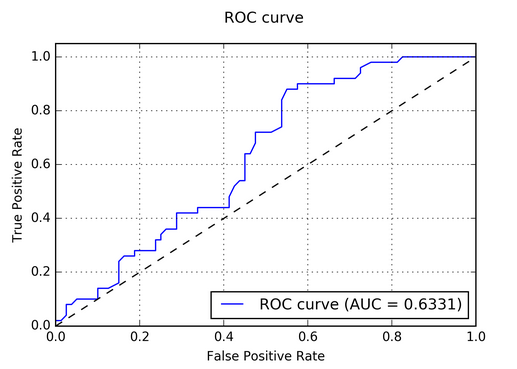
\includegraphics[width=0.5\textwidth]{ROC.png}
\caption{ROC curve associated to the slide base evaluation}
\label{Eval: ROC}
\end{figure}

The conference was held in Prague and I also attended a tutorial on deep neural networks that was given at the end of the conference. It lasted 4 days and to the surprise of some, histopathology is gaining in popularity as you could easily end up listening to only histopathology talks. In most histopathology talks, neural network, the state of the art in image processing were used and it seems, as I am focus in application, that it is essential for me to try and to apply deep convolutionnal network to my projects.


\section{May 2016 and future work}



%\begin{figure}[!ht]
%\centering
%\includegraphics[width=\textwidth]{}
%\caption{}
%\label{}
%\end{figure}

\section*{Results}
\begin{table}[!ht]
\centering
\begin{footnotesize}
\begin{tabular}{llllrrrr}
\toprule
 n\_tree    &  m\_try  & n\_bootstrap     &  n\_subsampling    &  Precision &     Recall &         F1 &   Accuracy \\
\midrule
1000 & 10 & 1000 & 2000 &            &            &            &            \\
     & 15 &      &      &       0.87 &       0.22 &       0.35 &       0.86 \\
     &    & 2000 &      &       0.86 &       0.20 &       0.32 &       0.85 \\
     & 20 & 1000 &      &       0.88 &       0.23 &       0.36 &       0.85 \\
     &    & 5000 &      &       0.64 &       0.12 &       0.20 &       0.84 \\
     & 30 & 2000 &      &       0.64 &       0.13 &       0.22 &       0.86 \\
     & 50 & 500 &      &       0.92 &       0.22 &       0.36 &       0.87 \\
     &    & 5000 &      &       0.88 &       0.22 &       0.35 &       0.85 \\
\textcolor{red}{500} & 10 & 1000 &      &       0.75 &       0.17 &       0.28 &       0.86 \\
     &    &      & 5000 &       0.82 &       0.08 &       0.14 &       0.84 \\
     &    & 10000 & 2000 &       0.69 &       0.02 &       0.03 &       0.84 \\
     &    &      & 5000 &       0.83 &       0.10 &       0.17 &       0.88 \\
     &    & 2000 & 2000 &       0.81 &       0.04 &       0.08 &       0.90 \\
     &    &      & 5000 &       0.88 &       0.28 &       0.40 &       0.85 \\
     &    & 500 & 2000 &       0.71 &       0.02 &       0.04 &       0.85 \\
     &    & 5000 &      &       0.85 &       0.23 &       0.33 &       0.84 \\
     &    &      & 5000 &       0.81 &       0.14 &       0.21 &       0.87 \\
     & 15 & 1000 & 2000 &       0.82 &       0.02 &       0.04 &       0.87 \\
     &    &      & 5000 &       0.85 &       0.31 &       0.43 &       0.84 \\
     &    & 10000 & 2000 &       0.95 &       0.05 &       0.10 &       0.83 \\
     &    &      & 5000 &       0.90 &       0.09 &       0.17 &       0.88 \\
     &    & 2000 & 2000 &       0.76 &       0.03 &       0.06 &       0.90 \\
     &    &      & 5000 &       0.85 &       0.14 &       0.22 &       0.85 \\
     &    & 500 & 2000 &       0.87 &       0.04 &       0.08 &       0.86 \\
     &    &      & 5000 &       0.89 &       0.12 &       0.20 &       0.84 \\
     &    & 5000 & 2000 &       0.83 &       0.03 &       0.06 &       0.83 \\
     &    &      & 5000 &       0.84 &       0.15 &       0.24 &       0.87 \\
     & \textcolor{red}{20} & \textcolor{red}{1000} & 2000 &       0.84 &       0.03 &       0.05 &       0.88 \\
     &    &      & \textcolor{red}{5000} &       \textcolor{red}{0.86} &       \textcolor{red}{0.33} &       \textcolor{red}{0.45} &       \textcolor{red}{0.84} \\
     &    & 10000 & 2000 &       0.84 &       0.04 &       0.08 &       0.86 \\
     &    &      & 5000 &       0.88 &       0.13 &       0.23 &       0.89 \\
     &    & 2000 & 2000 &       0.85 &       0.04 &       0.08 &       0.90 \\
     &    &      & 5000 &       0.88 &       0.13 &       0.21 &       0.86 \\
     &    & 500 & 2000 &       0.91 &       0.04 &       0.08 &       0.85 \\
     &    &      & 5000 &       0.90 &       0.21 &       0.32 &       0.85 \\
     &    & 5000 & 2000 &       0.94 &       0.05 &       0.09 &       0.82 \\
     &    &      & 5000 &       0.80 &       0.24 &       0.34 &       0.86 \\
     & 30 & 1000 & 2000 &       0.76 &       0.03 &       0.05 &       0.89 \\
     &    &      & 5000 &       0.88 &       0.14 &       0.22 &       0.85 \\
     &    & 10000 & 2000 &       0.82 &       0.03 &       0.06 &       0.86 \\
     &    &      & 5000 &       0.84 &       0.10 &       0.17 &       0.89 \\
     &    & 2000 & 2000 &       0.86 &       0.03 &       0.06 &       0.89 \\
     &    &      & 5000 &       0.87 &       0.12 &       0.20 &       0.86 \\
     &    & 500 & 2000 &       0.91 &       0.07 &       0.13 &       0.88 \\
     &    &      & 5000 &       0.89 &       0.18 &       0.29 &       0.83 \\
     &    & 5000 & 2000 &       0.91 &       0.09 &       0.16 &       0.88 \\
     &    &      & 5000 &       0.83 &       0.15 &       0.23 &       0.87 \\
     & 50 & 1000 & 2000 &       0.82 &       0.04 &       0.07 &       0.89 \\
     &    &      & 5000 &       0.90 &       0.12 &       0.20 &       0.85 \\
     &    & 10000 & 2000 &       0.87 &       0.06 &       0.10 &       0.86 \\
     &    &      & 5000 &       0.82 &       0.11 &       0.18 &       0.89 \\
     &    & 2000 & 2000 &       0.77 &       0.03 &       0.06 &       0.90 \\
     &    &      & 5000 &       0.88 &       0.18 &       0.27 &       0.86 \\
     &    & 500 & 2000 &       0.81 &       0.06 &       0.10 &       0.88 \\
     &    & 5000 &      &       0.88 &       0.24 &       0.35 &       0.82 \\
     &    &      & 5000 &       0.82 &       0.19 &       0.28 &       0.87 \\
\bottomrule

\end{tabular}
\end{footnotesize}
\caption{Performance estimated for our type of random forests by cross validation (10-fold)}
\label{Cross_val: RF}
\end{table}
\newpage

\bibliographystyle{unsrt} %% ou autre style

\bibliography{biblio.bib}





\end{document}



%%%%%%%%%%%%%%%%%%%%%%%%%%%%%%%%%%%%%%%%%%%%%%%%%%%%%%%%%%%%%%%%%%%%